%\clearpage
\section{Fairness Influence Functions (FIF)}
Now, we present an elaborate discussion on computing fairness influence functions.
A Fairness Influence Function, denoted as $ \mathsf{FIF}(\cdot) $, is computed with respect to a \textit{quantity of interest}, for example, the  PPV of the classifier or different fairness metrics such as DI and SP. Let $ \mathbf{S}  \subseteq \nonsensitive $ be a set of non-sensitive features, for which we are interested in computing their influence. A general approach to compute $ \mathsf{FIF}(\mathbf{S}) $ is to replace each feature in $ \mathbf{S} $ with random values and report differences in the quantity of interest~\cite{datta2016algorithmic}. Let $ \mathcal{X}'_i $ denote the modified marginal distribution where we replace feature $ X_i \in \mathbf{S} $ with random values. For example, $ \mathcal{X}'_i $ can be viewed as an uniform distribution within the support of $ X_i $. We then define the modified product distribution, denoted as $ \mathcal{D}_{-\mathbf{S}} $ by combining all marginal distributions, where each feature in $ \mathbf{S} $ has a modified distribution. 
\[
\mathcal{D}_{-\mathbf{S}} = \prod_{i | X_i \in \mathbf{S}} \mathcal{X}'_i \prod_{i | X_i \in X \setminus \mathbf{S}} \mathcal{X}_i \prod_{j=1}^{n} \mathcal{A}_j 
\]
We first give a general definition of influence function of $ \mathbf{S} $ on a quantity, say $ Q $, in the following. 
\[
\mathsf{FIF}(\mathbf{S}) \triangleq Q(\mathcal{D}) - Q(\mathcal{D}_{-\mathbf{S}})
\]
Intuitively, influence of $ \mathbf{S} $ is the difference in a quantity computed for the original distribution $ \mathcal{D} $ and the modified distribution $ \mathcal{D}_{-\mathbf{S}} $. In the following, we define influence function in terms of PPV of the classifier. 
\[
\mathsf{FIF}_{\mathsf{PPV}}(\mathbf{S}) \triangleq \Pr[\hat{Y} = 1 | \mathcal{D}] - \Pr[\hat{Y} = 1 | \mathcal{D}_{-\mathbf{S}}]
\]
Influence function also generalizes to PPV specific to compound sensitive groups. For a sensitive group $ \mathbf{a} \in \sensitive $, we define group-specific influence as follows. 

\[
\mathsf{FIF}_{\mathsf{PPV},\; \mathbf{a}}(\mathbf{S}) \triangleq \Pr[\hat{Y} = 1 | \sensitive = \mathbf{a}, \mathcal{D}] - \Pr[\hat{Y} = 1 | \sensitive = \mathbf{a},  \mathcal{D}_{-\mathbf{S}}]
\]

\paragraph{Experimental Analysis.} We empirically instantiate computation of FIF and its consequences for a logistic regression classifier on COMPAS and Adult datasets.

For both the datasets, we consider biological `sex' as the sensitive features.
In both cases, we denote the sensitive groups `male' and `female' as `sex=0' and `sex=1', respectively. 
FIFs computed for these sensitive groups show influence of different features and their relevant disparities. We illustrate the results in Figure~\ref{fairness_fvgm_fig:fif}.

Figure~\ref{fairness_fvgm_fig:fif_a} illustrates that the PPV value for the `male' population in the dataset is $0.61$. If we now replace the feature `age' with uniformly random values, the PPV for the same group becomes $0.46$, Thus, the FIF of the feature `age' for `male' group is $0.15$.
Similarly, all the red bars in Figures~\ref{fairness_fvgm_fig:fif_a}-\ref{fairness_fvgm_fig:fif_b}, ~\ref{fairness_fvgm_fig:fif_c}-\ref{fairness_fvgm_fig:fif_d} indicate a positive influence of that feature and the green bars indicate a negative influence of the feature on the individual getting classified to $\hat{Y}=1$.

In Figures~\ref{fairness_fvgm_fig:fif_c} and~\ref{fairness_fvgm_fig:fif_f}, we illustrate the influence of different features on the disparate impact between the two groups `male' and `female'. 
The green bar indicates that removing a feature causes an increase in DI, i.e. fairness in classification, and the red bar indicates the opposite. Alternatively, we can conclude that bigger is the green bar for a feature, higher is the bias-inducing effect of it.

Thus, from Figure~\ref{fairness_fvgm_fig:fif_c}, we conclude that `age' is the most bias-inducing feature among the two groups `male' and `female'.
From Fig~\ref{fairness_fvgm_fig:fif_a} and~\ref{fairness_fvgm_fig:fif_b}, we observe that `age' is a decisive feature for `male' while it is comparatively insignificant for `female'.

In case of Adult dataset, the PPV for `male' and `female' groups are 0.45 and 0.3 respectively. Among all the features, we observe that `race' has a positive impact on the classification for both the groups. This means removing the `race' information decreases the chance of getting classified to higher economic group. On the other hand, `capital-gain' has the highest influence on the classification for both groups. It is also the most biased-inducing feature as it varies most disparately among the two groups as the `capital-gain' differs significantly between two groups. 
\begin{figure}
	\begin{center}
	
		\subfloat[COMPAS]{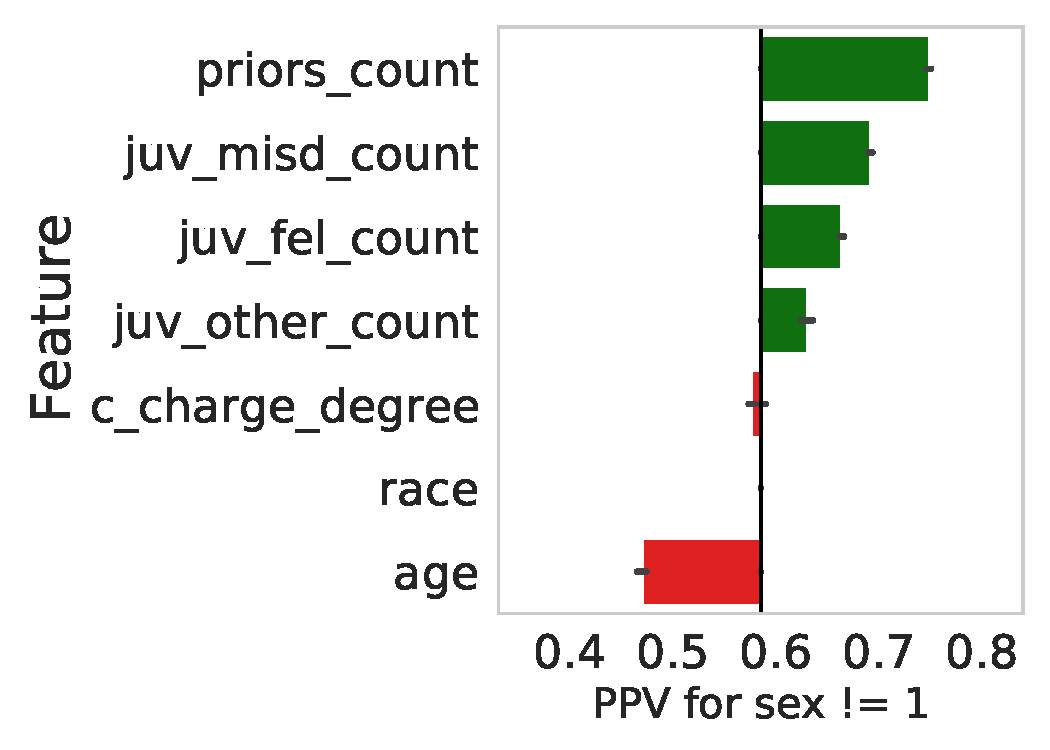
\includegraphics[scale=0.35]{figures/fairness/fvgm/dependency_exp_Learn-dependency_compas_lr_sex_0}\label{fairness_fvgm_fig:fif_a}}
		\subfloat[COMPAS]{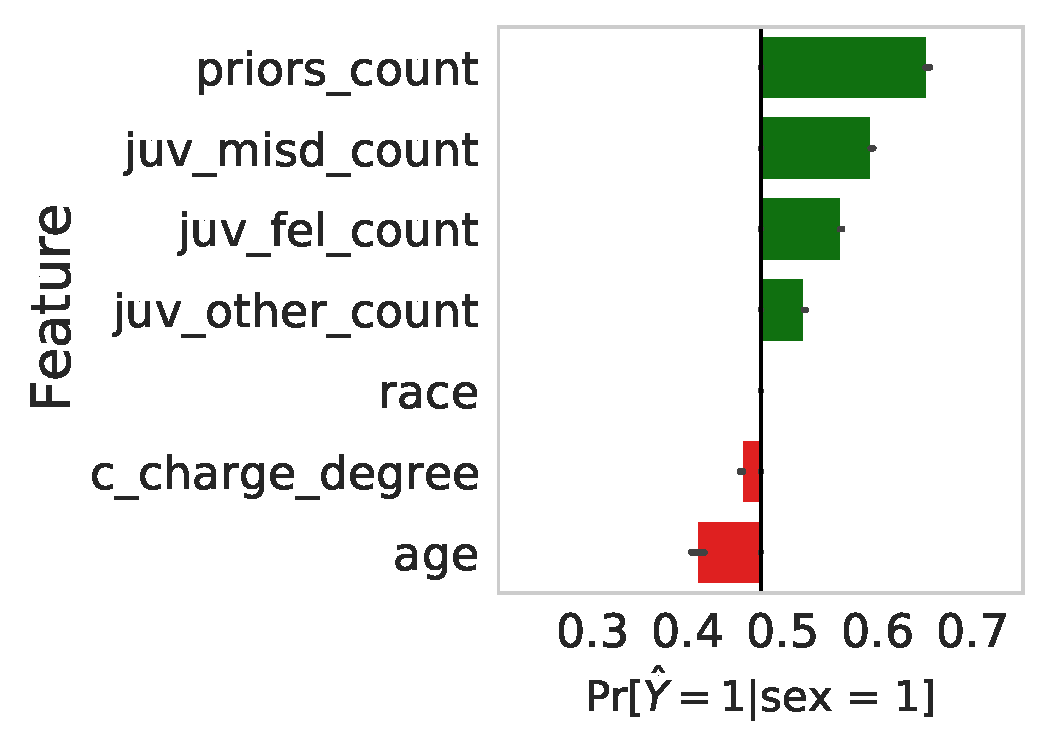
\includegraphics[scale=0.35]{figures/fairness/fvgm/dependency_exp_Learn-dependency_compas_lr_sex_1}\label{fairness_fvgm_fig:fif_b}}\\
		\subfloat[Adult]{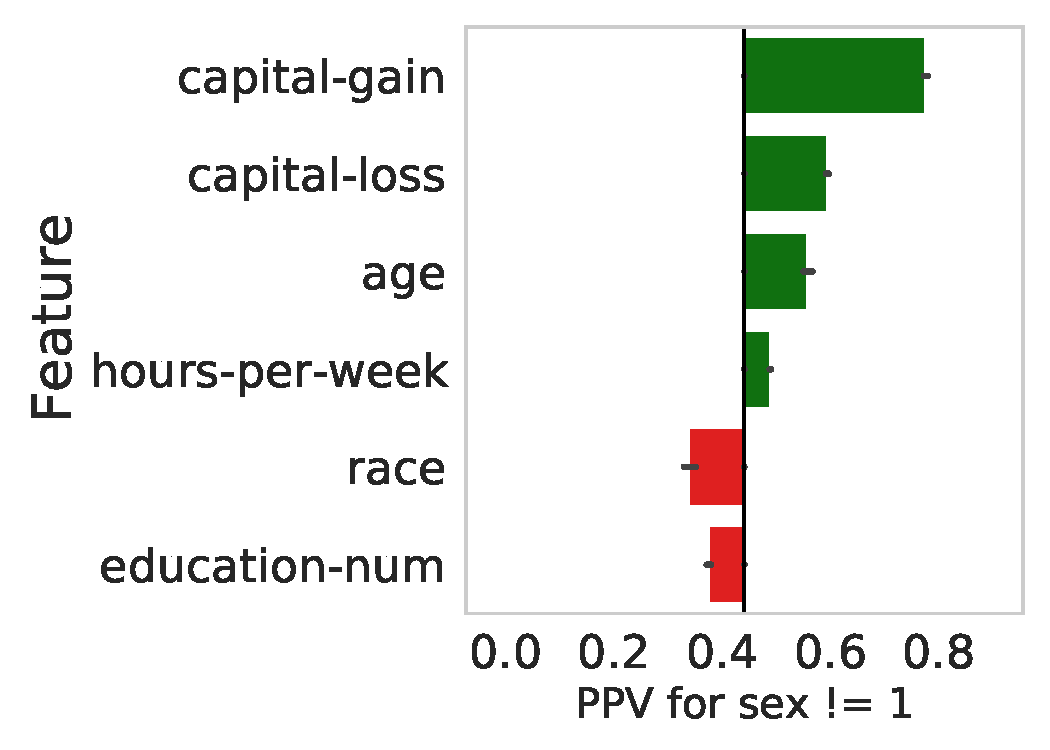
\includegraphics[scale=0.35]{figures/fairness/fvgm/dependency_exp_Learn-dependency_adult_lr_sex_0}\label{fairness_fvgm_fig:fif_d}}
		\subfloat[Adult]{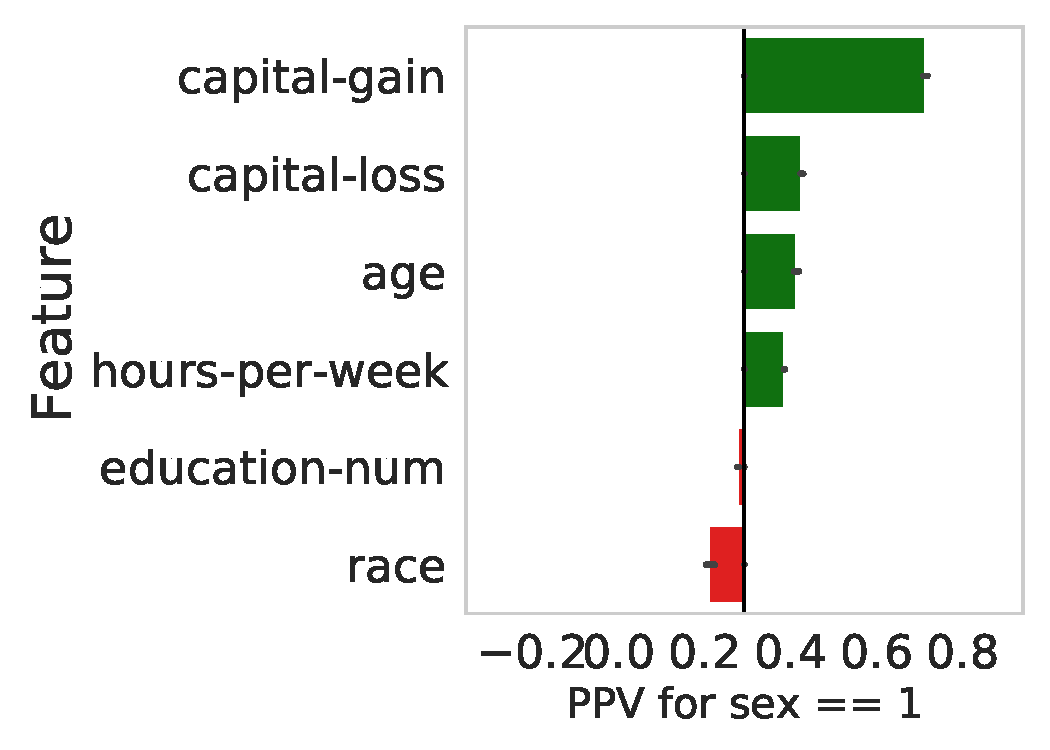
\includegraphics[scale=0.35]{figures/fairness/fvgm/dependency_exp_Learn-dependency_adult_lr_sex_1}\label{fairness_fvgm_fig:fif_e}}\\
		\subfloat[COMPAS]{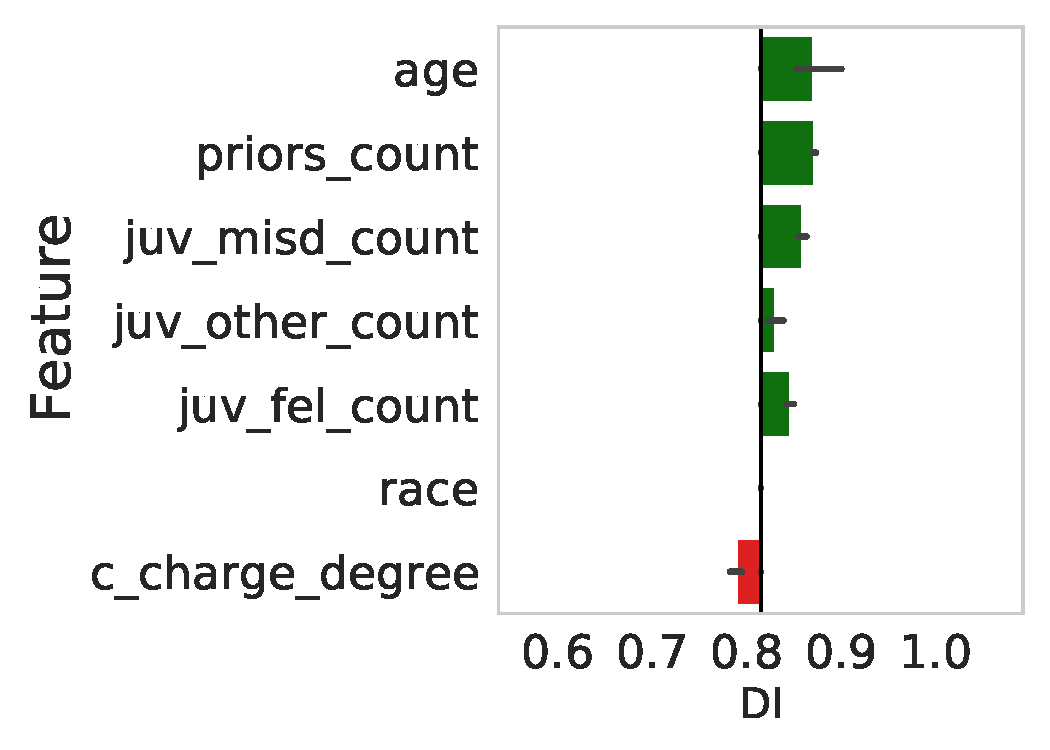
\includegraphics[scale=0.35]{figures/fairness/fvgm/dependency_exp_Learn-dependency_compas_lr_sex_DI}\label{fairness_fvgm_fig:fif_c}}
		\subfloat[Adult]{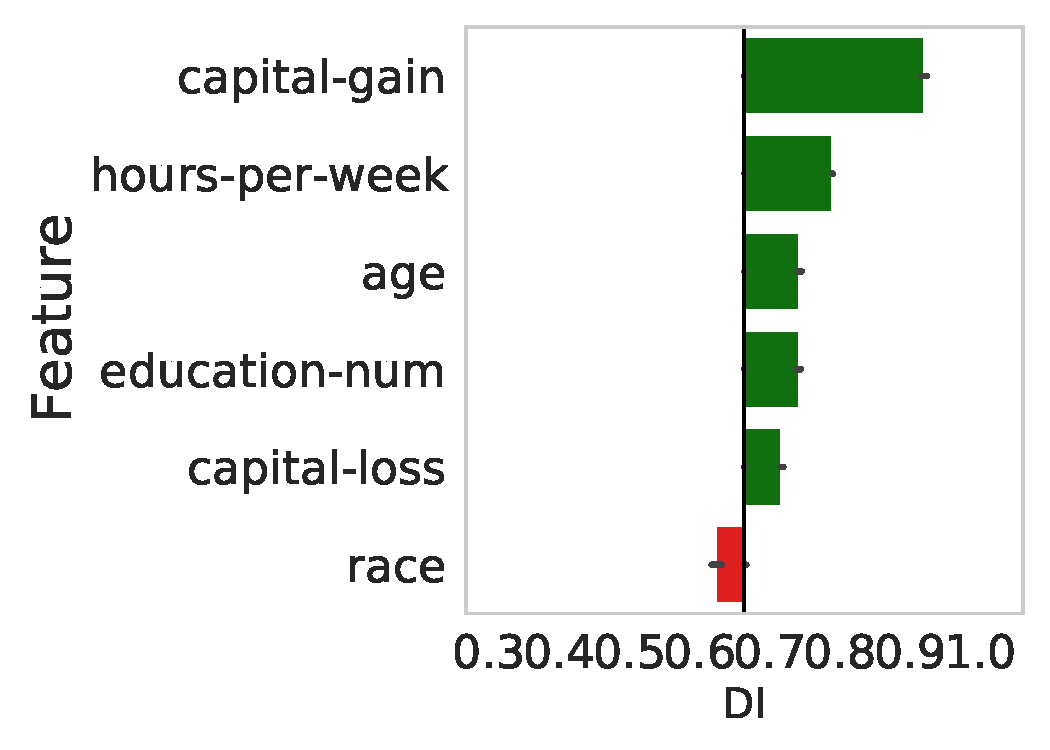
\includegraphics[scale=0.35]{figures/fairness/fvgm/dependency_exp_Learn-dependency_adult_lr_sex_DI}\label{fairness_fvgm_fig:fif_f}}\\
		
	
		
	\end{center}
	\caption[FIF illustration using {\fvgm}]{Extended results on computing feature influence functions (FIF) for COMPAS  and Adult dataset.}\label{fairness_fvgm_fig:fif}
\end{figure}


